\chapter{Les lentilles}

\section{Propagation dans les diélectriques}
\begin{wrapfigure}[10]{l}{5.5cm}
	\vspace{-5mm}
	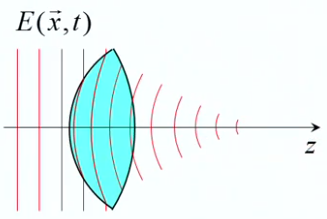
\includegraphics[scale=0.45]{ch3/image1.png}
	\captionof{figure}{ }
	\end{wrapfigure}	
Les lentilles étant faites en matériau diélectriques, il est intéressant de s'y attarder. Un diélectrique 
est un milieu constitués d'atomes qui conservent leurs électrons (à la différence des conducteurs). Si on 
place un atome dans un champ électrique, les deux vont se de façon opposés (étant de charge opposée) sur 
un distance $x(t)$ (le champ électrique dépendant du temps). Ceci donne lieu à un dipôle oscillant.\\

\begin{wrapfigure}[6]{r}{9cm}
	\vspace{-5mm}
	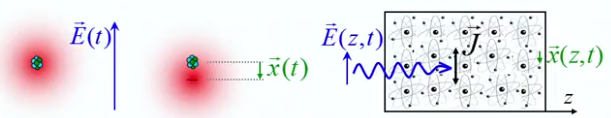
\includegraphics[scale=0.45]{ch3/image2.png}
	\captionof{figure}{ }
	\end{wrapfigure}
Dans un matériau diélectrique, on aura une vibration $\vec{x}(z,t)$ où $z$ est la coordonnée de propagation. 
Ceci donne lieur à des mouvements de charges dépendant de la position et du temps. Comme ces charges bougent, 
elles créent une densité de courant. On définit ainsi la \textit{densité de courant des charges liées}
\begin{equation}
\vec{J} = \eta_aq\dfrac{\partial \vec{x}}{\partial t}
\end{equation}
L'idée est d'aborder ça avec les équations de Maxwell
\begin{equation}
\left\{\begin{array}{ll}
\rot \vec{E} &= -\dfrac{\partial \vec{B}}{\partial t}\\
\rot \vec{B} &= \mu_0\vec{J} + \mu_0\epsilon_0\dfrac{\partial \vec{E}}{\partial t}
\end{array}\right.
\end{equation}
En prenant le rotationnel de la première équation
\begin{equation}
\rot(\rot\vec{E}) = -\dfrac{\partial \rot\vec{B}}{\partial t} = -\mu_0\dfrac{\partial \vec{J}}{\partial 
t} - \mu_0\epsilon_0\dfrac{\partial^2\vec{E}}{\partial t^2}
\end{equation}
La divergence étant nulle, le rotationnel du rotationnel donne $-\Delta$ ce qui donne, après simplification 
des signes négatifs
\begin{equation}
\Delta \vec{E} = \mu_0\dfrac{\partial\vec{J}}{\partial t}+\mu_0\epsilon_0\dfrac{\partial^2\vec{E}}{\partial 
t^2}
\end{equation}
En considérant le cas à une dimension en en faisant passer le second terme dans le membre de gauche :
\begin{equation}
\dfrac{\partial^2\vec{E}}{\partial z^2} - \dfrac{1}{c^2}\dfrac{\partial^2\vec{E}}{\partial t^2} = \mu_0 
\dfrac{\partial\vec{J}}{\partial t}
\end{equation}
On retrouve exactement l'équation d'onde sans le terme de densité de courant de charges liées : le milieu 
introduit un terme en $\vec{J}$ un peu comme un terme de source. Avec l'expression de $\vec{J}$ :
\begin{equation}
\dfrac{\partial^2\vec{E}}{\partial z^2} - \dfrac{1}{c^2}\dfrac{\partial^2\vec{E}}{\partial t^2} = \mu_0 \eta_a 
q \dfrac{\partial^2\vec{x}}{\partial t^2}
\end{equation}

\begin{wrapfigure}[8]{l}{4cm}
	\vspace{-2mm}
	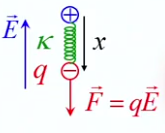
\includegraphics[scale=0.55]{ch3/image3.png}
	\captionof{figure}{ }
	\end{wrapfigure}
On voit apparaître l'accélération des charges et non pas un mouvement de translation qui génère des ondes. 
Notons que $\vec{x}$ est bien fonction du champ : comment $\vec{x}$ évolue en fonction du champ. Ceci 
permettra de "fermer" l'équation et ainsi de la résoudre. Pour se faire, adoptons le modèle des ressorts 
de Lorentz : le nuage électronique est lié aux noyaux comme une masse fixée à un ressort. Il est dès lors 
possible de lier ces deux variables. En faisant ceci, on réalise que l'on peut obtenir la solution suivante\footnote{
Les détails ne sont pas repris ici, c'est du rappel (cf. BA1).}
\begin{equation}
E(z,t) = E_\omega \cos[k(\omega)z-\omega t]
\end{equation}
La seule différence par rapport à la propagation dans le vide est que l'expression $k(\omega)$ est non 
triviale (dans le vide $k=\omega/c$). La résolution de l'équation d'onde (dérivée double par rapport à 
$z$) donne lieu à
\begin{equation}
k^2=\dfrac{\omega^2}{c^2}+\omega^2\mu_0\epsilon_0\chi(\omega) = \dfrac{\omega^2}{c^2}[1+\chi(\omega)]
\end{equation}
où $\chi(\omega)$ est la susceptibilité du milieu. Cette simple fonction contient l'information relative 
au movement des charges dans le diélectrique. En utilisant la \textit{perméabilité relative du mileu} 
$\epsilon_r = [1+\chi(\omega)]$, on peut écrire
\begin{equation}
k(\omega) = \dfrac{\omega}{c}\sqrt{\epsilon_r(\omega)} = \dfrac{\omega}{c} n(\omega)
\end{equation}
où $n(\omega) \equiv \sqrt{\epsilon_r(\omega)}$ est l'indice de réfraction. Il s'agit d'une fonction 
qui contient toute la dynamique des charges mises en mouvement par le champ électrique lui même, elle 
reforme toute la complexité microscopique. On peut montrer que $c/n(\omega)$ est la \textit{vitesse de 
propagation (phase) de la lumière dans un diélectrique}\footnote{Pour le voir, mettre $k(\omega)$ en évidence 
dans la solution de l'équation d'onde $E(z,t)$.}
\begin{equation}
\hookrightarrow k(\omega) = \dfrac{\omega}{c}\sqrt{\epsilon_r(\omega)} = \dfrac{\omega}{c} n(\omega) = 
\dfrac{\omega}{v}
\end{equation}
L'indice de réfraction est le facteur de diminution de la vitesse de l'onde dans un diélectrique, 
l'indice de réfraction étant toujours plus grande que l'unité.
\begin{equation}
v = \frac{c}{n}
\end{equation}


Tout se base la dessus. Étudions une lame de matériau diélectrique (verre) traversée par une onde 
plane monochromatique :
\begin{equation}
E(z,t) = E_\omega \cos[kz-\omega t]
\end{equation}
\newpage
\begin{wrapfigure}[8]{l}{6.4cm}
%	\vspace{-2mm}
	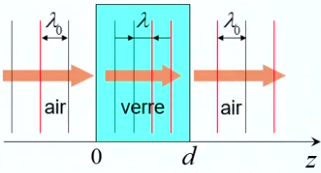
\includegraphics[scale=0.55]{ch3/image4.png}
	\captionof{figure}{ }
	\end{wrapfigure}
Avant de rentrer dans la lentille, l'onde plane se propage dans le vide : $k= k_0$ soit le 
nombre d'onde dans le vide et $\lambda_0 = \frac{2\pi}{k_0}$ la longueur d'onde dans le vide. Dans 
le milieu diélectrique, il ne faut \textbf{pas} reprendre $k_0$ mais $k = k_0n$ : la longueur 
d'onde sera plus petite, divisée par $n$, l'indice de réflexion est également le facteur de diminution 
de la longueur d'onde : $\lambda = \lambda_0/n$. \\

Interprétons ceci en nous basant sur la vitesse dans le diélectrique 
\begin{equation}
v = \frac{\omega}{n} = \frac{\omega}{k_0n} = \frac{c}{n}
\end{equation}

\begin{wrapfigure}[8]{r}{6.4cm}
	\vspace{-10mm}
	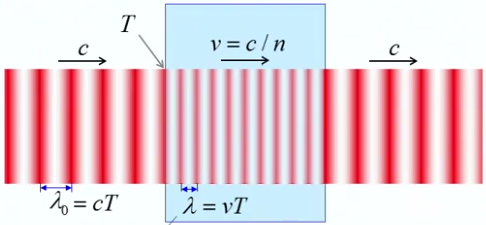
\includegraphics[scale=0.35]{ch3/image5.png}
	\captionof{figure}{Dans le vide $\lambda_0=cT$ et dans le verre $\lambda = vT$.}
	\end{wrapfigure}
La vitesse dans le diélectrique est moindre (les fronts d'ondes paraissent plus rapprochés), mais la 
période reste bien sûr inchangée. Le 
diélectrique cause un \textit{déphasage} : dans le diélectrique un front d'onde va "moins loin" que 
s'il était dans le vide (les fronts d'ondes seraient plus espacés), il y a donc distorsion de phase.\\


\begin{wrapfigure}[6]{l}{4.4cm}
	\vspace{-5mm}
	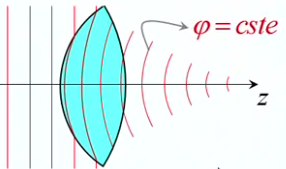
\includegraphics[scale=0.35]{ch3/image6.png}
	\captionof{figure}{ }
	\end{wrapfigure}
Une lentille c'est une lame à épaisseur variable causant un retard de phase variable (plus l'épaisseur 
de verre traversée est grande, plus cet effet de déphasage sera important). Les lieux de points de phases 
constantes, les fronts d'ondes, seront des surfaces à priori courbes.\\

Comme nous nous intéressons à la phase, aux fronts d'onde, regardons le phaseur
\begin{equation}
E(z,t) = E_\omega e^{ikz}e^{-i\omega t}
\end{equation}
La phase accumulée sur l'épaisseur $d$ sera forcément $\varphi = kd = nk_0d$. Sans la lame de verre 
$\varphi = k_0d$. Le \textit{retard de phase (déphasage)} est obtenu en comparant la phase accumulée 
dans le verre avec celle dans le vide pour la même longueur traversée c'est à dire $d$
\begin{equation}
\Delta\varphi = k_0d(n-1)
\end{equation}
\textbf{Remarque} : un retard de phase est une phase qui évolue plus vite dans le diélectrique, mais 
il faut se souvenir que pour une distance donnée on a une "plus grande densité de fronts d'onde". Phase 
qui évolue rapidement veut dire retard de phase.\\


\newpage
\section{Fonction de transfert d'une lentille "mince"}
Le terme \textit{mince} a été introduit pour faire plusieurs approximation, on verra ça plus tard ! Le 
but de la fonction de transfert est de connaître le champ transmis par un simple produit avec le champ 
incident.
\begin{equation}
E_t(\vec{x}) = T(x,y)\times E_i(\vec{x})
\end{equation}

	\subsection{Lentilles à surfaces sphériques}
	\begin{wrapfigure}[7]{l}{4.4cm}
	\vspace{-5mm}
	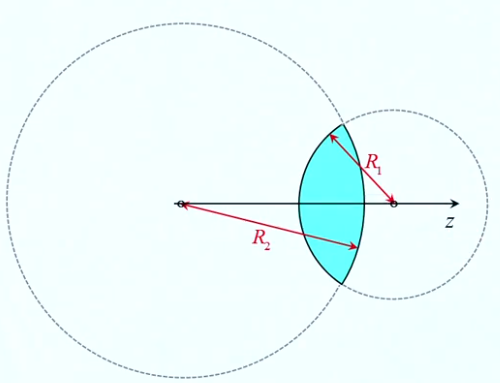
\includegraphics[scale=0.2]{ch3/image7.png}
	\captionof{figure}{ }
	\end{wrapfigure}
	L'idée d'une telle surface est que la surface est constituée de "morceau de surface de sphère", 
	la lentille peut être vue comme l'intersection de deux sphères. On nomme l'axe $z$ 
	l'\textit{axe optique} (axe reliant le centre des deux sphères) de la lentille (voir ci-contre). 
	L'épaisseur est variable en fonction de la position dans le plan transverse : son épaisseur 
	maximale est nommée $\Delta_0$.\\
	
	\begin{wrapfigure}[9]{r}{4.4cm}
	\vspace{-5mm}
	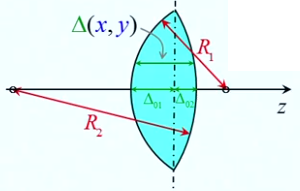
\includegraphics[scale=0.4]{ch3/image8.png}
	\captionof{figure}{ }
	\end{wrapfigure}
	Pour l'analyse, décomposons la lentille en deux : $\Delta_0 = \Delta_{01}+\Delta_{02}$. Ceci est 
	pour la hauteur maximale, mais on peut faire de même pour toute épaisseur
	\begin{equation}
	\Delta (x,y) = \Delta_1(x,y) + \Delta_2(x,y)
	\end{equation}
	Commençons par décrire la fonction $\Delta_1(x,y)$. Considérons un point du plan transverse $(x,y)$. 
	On se situe à $R_1$ du centre de courbure, que vaut cette épaisseur ? Faisons un peu de géométrie. 
	La distance de l'axe optique vaut $\sqrt{x^2+y^2}$ et celle depuis le centre de courbure vaut 
	$\sqrt{R_1^2-x^2-y^2}$ (par Pythagore). La distance entre l'extérieur de la lentille et la 
	coordonnée en $z$ de $(x,y)$ vaut $R_1-\sqrt{R_1^2-x^2-y^2}$. Pour exprimer $\Delta_1$, il suffit 
	de retirer à $\Delta_{01}$ cette distance que nous venons de calculer
	\begin{equation}
	\Delta_1(x,y) = \Delta_{01}-\left[ R_1-\sqrt{R_1^2-x^2-y^2}\right]
	\end{equation}
	De façon similaire, on trouve
	\begin{equation}
	\Delta_1(x,y) = \Delta_{02}-\left[ R_2-\sqrt{R_2^2-x^2-y^2}\right]	
	\end{equation}

	\begin{wrapfigure}[9]{l}{6.4cm}
	\vspace{-5mm}
	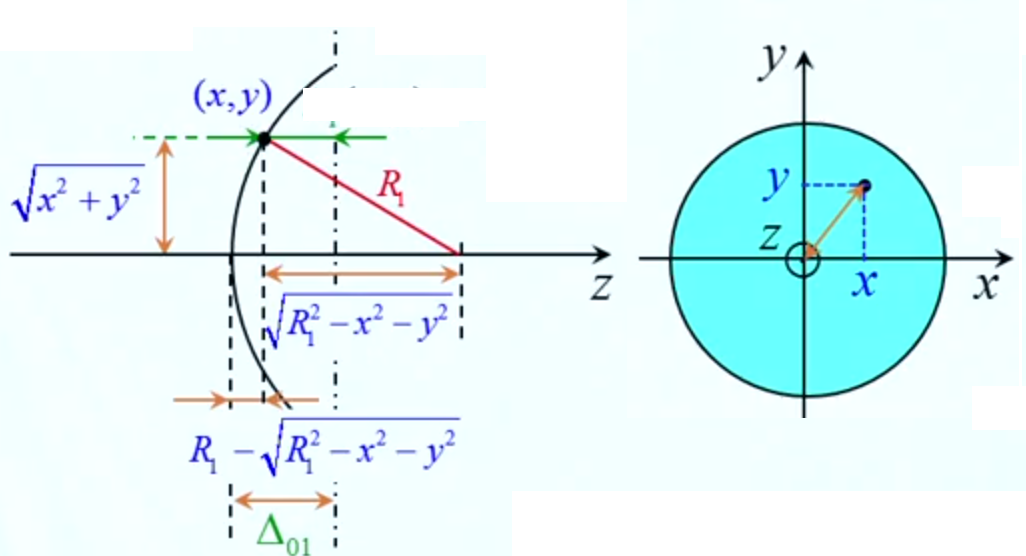
\includegraphics[scale=0.18]{ch3/image9.png}
	\captionof{figure}{ }
	\end{wrapfigure}	
	Comme nous l'avons précisé, nous allons considérer des lentilles \textit{minces} : fondamental 
	pour simplifier ces expressions. Il s'agit d'une lentille dont les rayons de courbures sont 
	très importants. Une lentille est mince lorsque sa distance transverse (taille de la lentille) 
	est petite par rapports aux rayons de courbures de ses surfaces 
	\begin{equation}
	\text{Lentilles "minces"} \qquad\Longrightarrow\qquad x^2+y^2 \ll R_1^2,R_2^2
	\end{equation}
	Il est dès lors possible d'utiliser l'approximation paraxiale/parabolique 
	\begin{equation}
	\Delta_1(x,y) = \Delta_{01}-\left[R_1-R_1\sqrt{1-\dfrac{x^2+y^2}{R_1^2}}\right] \approx \Delta_{01} -
	\left[R_1-R_1\left(1-\dfrac{x^2+y^2}{2R_1^2}\right)\right]
	\end{equation}
	En faisant les math
	\begin{equation}
	\begin{array}{ll}
	\Delta_1(x,y) &= \Delta_{01} - \dfrac{x^2+y^2}{2R_1}\\
	\Delta_2(x,y) &= \Delta_{02} - \dfrac{x^2+y^2}{2R_2}
	\end{array}
	\end{equation}
	La fonction $\Delta(x,y)$ est donnée en faisant la somme des deux termes
	\begin{equation}
	\Delta(x,y) = \Delta_0-\dfrac{x^2+y^2}{2}\left(\frac{1}{R_1}+\frac{1}{R_2}\right)
	\end{equation}
	
		\begin{wrapfigure}[9]{l}{6.4cm}
	\vspace{-5mm}
	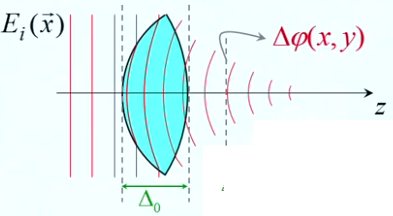
\includegraphics[scale=0.45]{ch3/image10.png}
	\captionof{figure}{ }
	\end{wrapfigure}	
	Cette expression permet d'étudier la fonction de transfert d'une lentille mince. Une lentille 
	propage des déphasages variables $\Delta \varphi(x,y)$. Afin de rester précis (la longueur d'onde 
	de la lumière étant petite, il vaut mieux), on va étudier 	les déphasages dans un plan $z$ précis : 
	le profil de phase $\Delta\varphi(x,y)$ sera donné pour un plan bien précis. On définit alors le plan 
	d'entrée (tangeant à la première surface) et de sortie (tangent à la seconde). 
	
	\subsection{Lentilles "minces"}
	La fonction de transfert relie la champ incident aux champs transmis dans ce second plan. Ces deux 
	plans sont séparés de $\Delta_0 \ll R_1,R_2$. Nous allons faire l'approximation que ces deux plans 
	sont tellement rapprochés que l'ont peu négliger la diffraction. Montrons le 
	\begin{equation}
	a(x,y;z) = \iint A(\rho,\sigma) e^{i\rho x}e^{i\sigma y} e^{i\sqrt{k^2-\rho^2-\sigma^2}z}\ d\rho d\sigma
	\end{equation}
	Dans le contexte de Fresnel (approximation paraxiale)
	\begin{equation}
	a(x,y;z) = \iint_{-\infty}^\infty A(\rho,\sigma)e^{i\rho x}e^{i\sigma y} e^{i\frac{\rho^2}{2k}z
	-i\frac{\sigma^2}{2k}z}\ d\rho d\sigma\ e^{ikz}
	\end{equation}
	Si on supprime les deux premières exponentielles de $z$ (le propagateur du spectre), on supprime 
	la diffraction
	\begin{equation}
	a(x,y;z) = \iint_{-\infty}^\infty A(\rho,\sigma)e^{i\rho x}e^{i\sigma y}\ d\rho d\sigma\ e^{ikz}
	\end{equation}
	Ceci est valable si $\max\rho$ est telle que $\max z = \Delta_0$
	\begin{equation}
	\frac{\rho^2}{2k}\Delta_0 \ll 1
	\end{equation}
	Admettons le pour le moment, on y reviendra. On a alors
	\begin{equation}
	a(x,y;z) = a(x,y;0)e^{ikz} = |a(x,y;0)|e^{i\varphi(x,y)}e^{ikz}
	\label{eq:amod}
	\end{equation}
	On retrouve un champ qui pris en module sera inchangé (le champ en $z$ sera le même que en 0). Le 
	propagateur à été réduit à son expression minimale : à une distance $z$ j'accumule une phase $kz$ quel 
	que soit le point du plan transverse dans lequel on se trouve. Cela correspond à une translation des 
	fronts d'onde comme illustré ci-dessous.
	
	\newpage

	\begin{wrapfigure}[8]{l}{6.4cm}
	\vspace{-3mm}
	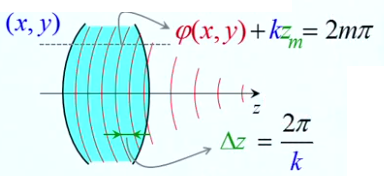
\includegraphics[scale=0.45]{ch3/image11.png}
	\captionof{figure}{ }
	\end{wrapfigure}		
	Regardons le lieu des points de phase constantes (de constante valant $2n\pi$)(def. front d'onde).
	Pour des valeurs de $x$ et $y$ fixé $\varphi(x,y) = c^{te}$ et on peut considérer que 
	l'équation ci-dessous, pour $x$ et $y$ donnés, donne les position en $z$ ou on trouve les 
	fronts d'onde.
	\begin{equation}
	\varphi(x,y) + kz_m = 2m\pi
	\end{equation}

	\begin{wrapfigure}[8]{r}{3.4cm}
	\vspace{-5mm}
	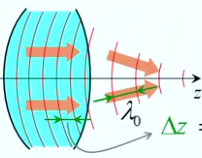
\includegraphics[scale=0.45]{ch3/image12.png}
	\captionof{figure}{ }
	\end{wrapfigure}				
	L'écart entre deux front d'onde est le même partout et vaut $\Delta z = 2\pi/k$, la longueur d'onde et 
	ce peut importe où on se situe. Ce n'est "normal" que si on supprime la diffraction. Il faut remarquer 
	que le $\Delta z$ est pris parallèlement à l'axe $z$ alors que l'on considère la longueur d'onde 
	perpendiculairement au front d'onde, les deux situations sont différentes. Dans la lentille on translate (rien 	    ne change entre 0 et $z$, pas de diffraction), alors que dans l'air le rayon de courbure devient de plus en plus petit (il y a en quelque sorte diffraction).\\

	Supposons que la variation du champ transverse incident se fait à une longueur caractéristique $\Delta l$. 
	On peut voir la lentille comme une fonction "fenêtre", limitant la taille du champ. C'est ce $\Delta l$ qui 
	va donner la valeur de $\rho$ pour étudier l'approximation. Pour se faire, regardons $A(\rho)$ la 
	transformée de Fourier de la fonction fenêtre, un sinc. La valeur maximal de $\rho$ vaut $\approx 2\pi/
	\Delta l$. Dans notre approximation
	\begin{equation}
	\frac{\rho^2}{2k}\Delta_0 \ll 1\qquad \Leftrightarrow\qquad \dfrac{4\pi^2\Delta_0}{2k\Delta l^2}\ll 1
	\end{equation}
	avec $k=2\pi/\lambda$ :
	\begin{equation}
	\Delta_0 \ll \dfrac{\Delta l^2}{\lambda}
	\end{equation}
	Il s'agit de l'inégalité inverse de celle de Fraunhofer : il fallait avoir une taille beaucoup plus grande 
	mais cette fois-ci comme la diffraction est négligée il faut être beaucoup plus petit.\\
	
	Pour exprimer la fonction de transfert, il faut exprimer le déphasage accumulé dans la lentille. Pour 
	un chemin optique $\Delta z$ parallèle à l'axe optique on peut facilement exprimer le déphasage. En effet 
	avec \autoref{eq:amod} 
	\begin{equation}
	\Delta\varphi = k\Delta z
	\end{equation}
	\begin{wrapfigure}[12]{l}{5.4cm}
	%\vspace{-5mm}
	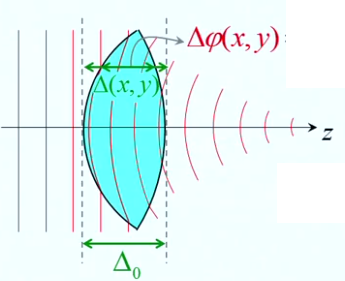
\includegraphics[scale=0.45]{ch3/image13.png}
	\captionof{figure}{ }
	\end{wrapfigure}		
	Dès lors, la phase accumulé dans la lentille vaudra simplement $\Delta \varphi(x,y) = k\Delta (x,y)$. 
	Comme on travaille sur la phase, il faut la définir pour une valeur de $z$ donnée (passage du plan 
	d'entrée au 	plan de sortie). Il faudra alors considérer la passage dans l'air, sans diffraction :
	\begin{equation}
	\Delta \varphi(x,y) = k\Delta (x,y) + k_0[\Delta_0-\Delta(x,y)]
	\end{equation}
	Il s'agit du déphasage introduit par la lentille en un point $(x,y)$ du plan transverse. Or, 
	$\Delta(x,y)$ est connu : à partir du champ dans le plan d'entrée $a(x,y)$ on pourra connaître le 
	champ $a'(x,y)$	dans le plan de sortie 
	\begin{equation}
	a'(x,y) = a(x,y)\underbrace{e^{i\Delta\varphi(x,y)}}_{T(x,y)}
	\end{equation}
	Le facteur de phase représente le déphasage accumulé du plan d'entrée au plan de sortie, y compris les 
	passages dans l'air. Attention, si la fonction de transfert ne contient que ceci, cela signifie que 
	que toute variation de l'amplitude du champ est négligée : l’absorption et les réflexion dans le 
	diélectrique sont négligées. Ceci définit la fonction de transfert $T(x,y)$.\\
	
	On peut écrire, en distribuant : $\Delta\varphi(x,y) = k_0\Delta_0 + (k-k_0)\Delta(x,y)$. Comme 
	$k=k_0n$, l'expression devient
	\begin{equation}
	\Delta\varphi(x,y) = k_0\left[\Delta_0+(n-1)\Delta(x,y)\right]
	\end{equation}
	En substituant l'expression de $\Delta(x,y)$ et après simplifications
	\begin{equation}
	\Delta \varphi(x,y) = k_0\left[n\Delta_0-(n-1)\dfrac{x^2+y^2}{2}\left(\dfrac{1}{R_1}+\dfrac{1}{R_2}\right)
	\right]
	\end{equation}
	Introduisons un nouveau paramètre
	\begin{equation}
	\frac{1}{f} \equiv (n-1)\left(\dfrac{1}{R_1}+\dfrac{1}{R_2}\right)
	\end{equation}
	afin d'écrire
	\begin{equation}
	\Delta\varphi(x,y) = k_0\left[n\Delta_0 - \dfrac{x^2+y^2}{2f}\right]
	\end{equation}
	Notre fonction de transfert devient alors
	\begin{equation}
	T(x,y) = e^{ik_0 n\Delta_0}\ e^{-i\frac{k_0}{2f}(x^2+y^2)}
	\end{equation}
	Le premier terme, de phase constante, revient à changer l'origine : on n'en tiendra pas compte ici (pas 
	d'interprétation physique si l'on n'étudie pas la dynamique de passage dans la lentille). On ne garde 
	que le terme de phase quadratique, ce qui est normal vu notre approximation parabolique. 
	\begin{equation}
	T(x,y) =\DS e^{\DS -i\frac{k_0}{2f}(x^2+y^2)}
	\end{equation}
	On verra que $f$ n'est que la \textit{distance focale} de la lentille (qui ne contient que l'indice de 
	réfraction et les rayons de courbures).
	
















